% DOCX paragraph 130.
\section{Experiments}
\label{sec:experiments}

% DOCX paragraph 131.
We evaluate AgentGS's overall performance and the contribution of its components through baseline comparisons and ablations. The experimental analysis also considers generalization to new combinations of existing capabilities and substitution of tools implementing the same capability, together with runtime costs. Finally, execution cases are used to examine performance differences and causes of failure. \drafttodo{generalization and runtime-cost results mentioned in the initial draft are to be supplied}.

% DOCX paragraph 132.
\subsection{Tasks and Experimental Setup}
\label{sec:experimental-setup}

% DOCX paragraph 133.
\paragraph{Data and evaluation scope.}
The main experiment uses all 603 GeoToolEval records. Ablations use a fixed subset of 57 records. All GeoToolEval experiments evaluate final answers with the FAS defined in Section~\ref{sec:metrics}, averaged over their respective evaluation sets with failures retained. To analyze workflow complexity, the main experiment additionally groups results by reference-chain length. The ablation subset is described in Section~\ref{sec:ablations}.

% DOCX paragraph 134. Model labels are retained as reported in the source.
\paragraph{Run configuration.}
We use GPT-5.6 Terra as the backbone and compute results from the raw records of AgentGS's first complete run over all 603 records, retaining both partial-credit and failed cases.

% DOCX paragraph 135.
\paragraph{Baselines.}
We compare scientific agents and language models. Agent baselines include GeoAgent~\cite{chen2024geoagent} and Earth-Agent~\cite{feng2026earthagent}. Both use GPT-5.6 Terra, as does AgentGS, to compare different agent systems with the same backbone. Language-model baselines include DeepSeek V4 Pro, GPT-5.6 Terra, GPT-5.4, Qwen-Plus, and GeoGPT. These compare direct language-model answers with answers obtained by agents using tools.

% DOCX paragraph 136.
\subsection{Main Results and Baseline Comparison}
\label{sec:main-results}

% DOCX paragraphs 137--139 and table 2.
Table~\ref{tab:main-results} reports mean FAS for AgentGS and the baselines. AgentGS achieves 0.8731, exceeding GeoAgent's 0.7804. It also outperforms the same GPT-5.6 Terra backbone answering directly, which scores 0.3137, and the other language-model baselines. We next analyze task strata and ablations to examine performance across tasks and the contributions of capability composition, hypergraph completion, and execution mechanisms.

\begin{table}[t]
\caption{GeoToolEval baseline comparison. AgentGS process metrics are per-record averages from the present 603-record end-to-end experiment; FAS values are retained from the source manuscript. Direct-answer language models have no tool traces; their process metrics are not applicable (---).}
\label{tab:main-results}
\centering
\begin{tabularx}{\columnwidth}{@{}Xrrr@{}}
\toprule
Method & FAS & TSF1 & TOS \\
\midrule
AgentGS (GPT-5.6 Terra) & \textbf{0.8731} & 0.9170 & 0.9166 \\
GeoAgent (GPT-5.6 Terra) & 0.7804 & 0.8663 & 0.7911 \\
EarthAgent (GPT-5.6 Terra) & 0.0862 & 0.1182 & 0.1390 \\
DeepSeek V4 Pro & 0.5162 & --- & --- \\
GPT-5.6 Terra & 0.3137 & --- & --- \\
GPT-5.4 & 0.3069 & --- & --- \\
Qwen-Plus & 0.2918 & --- & --- \\
GeoGPT & 0.2500 & --- & --- \\
\bottomrule
\end{tabularx}
\end{table}


% DOCX paragraph 140.
\paragraph{Task complexity and domain differences.}
Grouped by reference-chain length, AgentGS achieves mean FAS values of 0.9425 for single-step tasks, 0.7557 for two- to three-step tasks, and 0.6167 for tasks with at least four steps. Figure~\ref{fig:performance} reports results by domain. Longer chains are concentrated in remote sensing, creating overlap between chain-length and domain factors. Performance differences should therefore be interpreted using both groupings.

% DOCX paragraph 141 and embedded image 4.
\begin{figure*}[t]
  \centering
  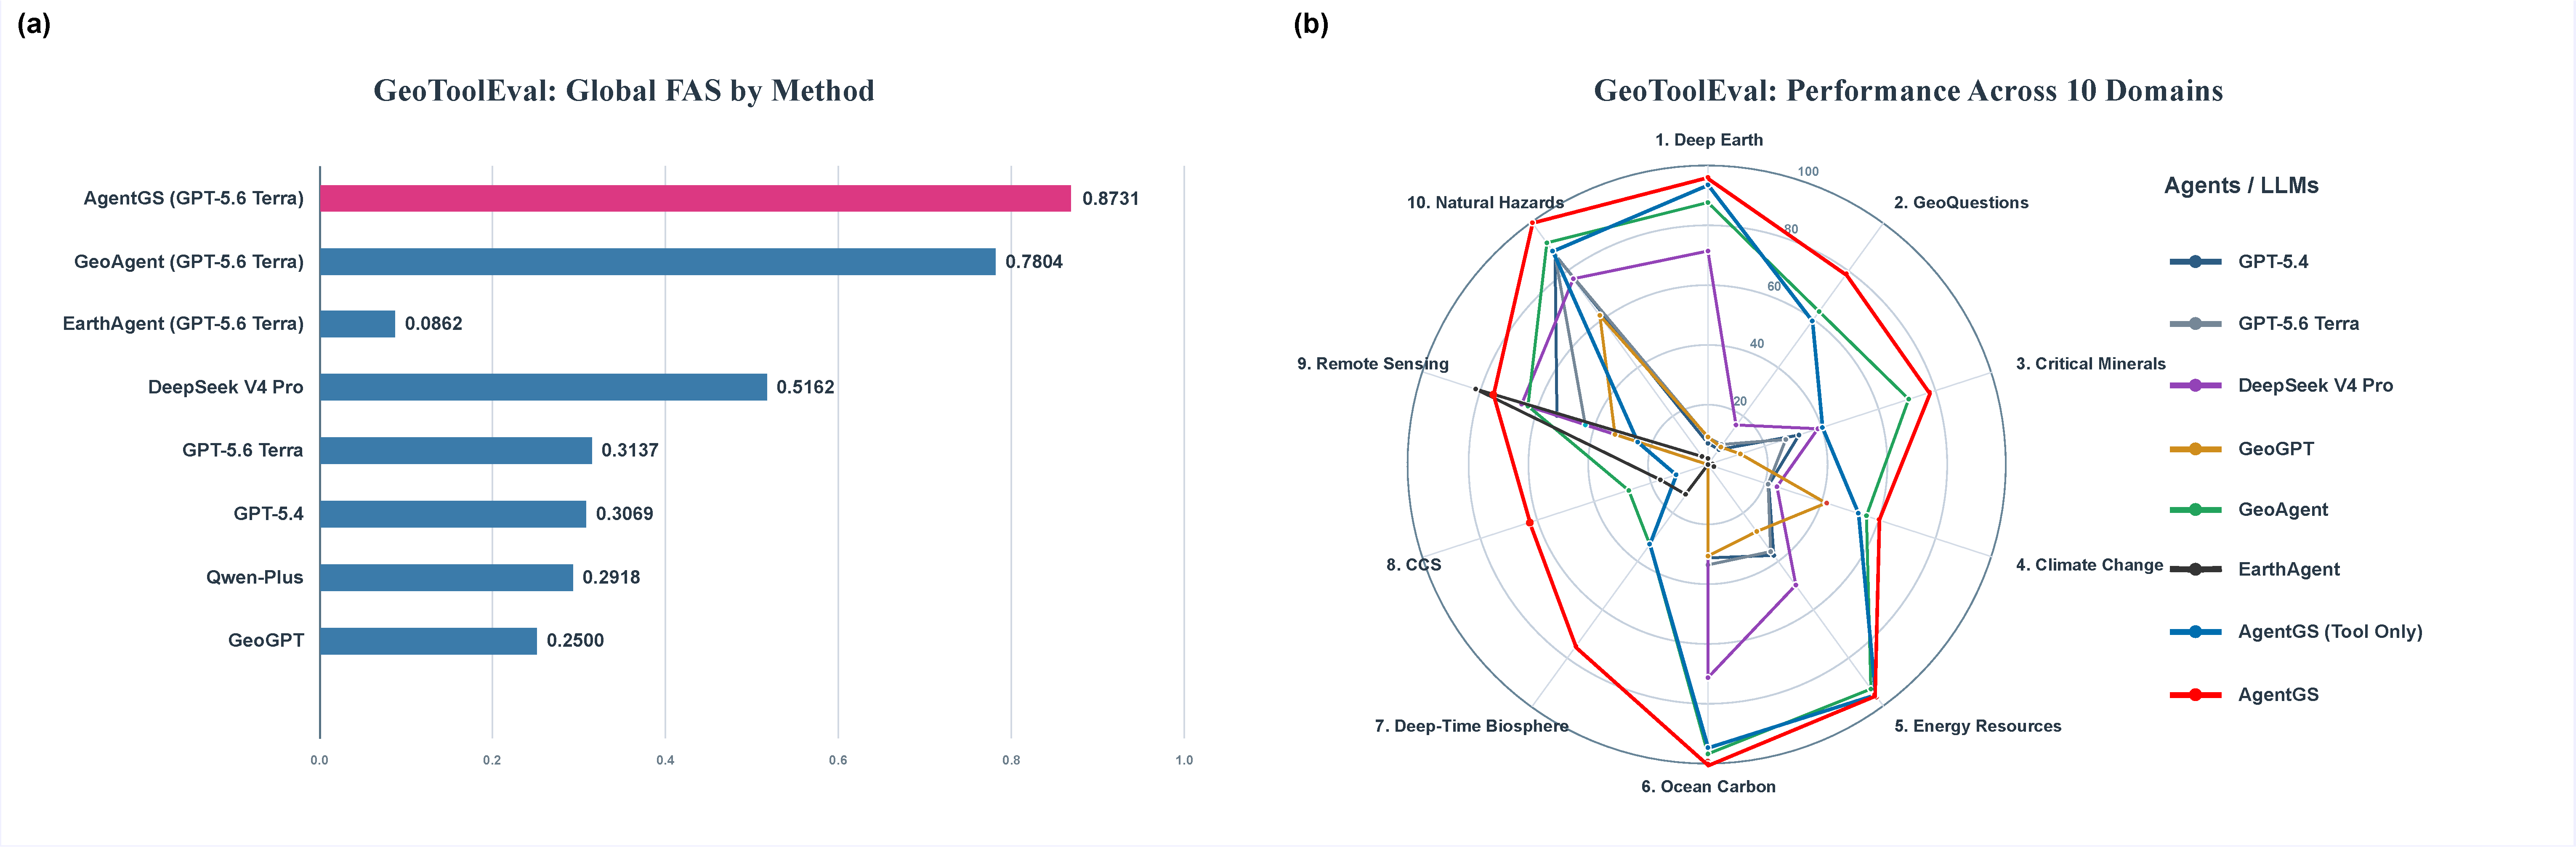
\includegraphics[width=\textwidth]{performance.pdf}
  \caption{Overall and domain-specific performance of AgentGS and baselines on GeoToolEval: (a) mean FAS across all evaluation records; (b) mean FAS across the ten geoscientific domains.}
  \label{fig:performance}
  \Description{A horizontal bar chart compares mean FAS for AgentGS, two agent baselines, and five language models. A radar chart presents performance across ten geoscientific domains.}
\end{figure*}


% DOCX paragraph 143.
\subsection{External Evaluation on GeoBenchX}
\label{sec:external-evaluation}

% DOCX paragraph 144.
To assess applicability in a different tool environment, we conduct an external evaluation on GeoBenchX~\cite{krechetova2025geobenchx}. We integrate its official tool set and separately construct corresponding Skills and Capabilities. Capabilities are defined from tool functions and input/output requirements, strategy dependencies are organized, and tool mappings are established. AgentGS then performs task planning and tool orchestration.

% DOCX paragraph 145. All experimental fields below were placeholders in the source.
The experiment uses \drafttodo{number of tasks} tasks and compares against \drafttodo{baseline method}. AgentGS and the baseline use \drafttodo{AgentGS backbone and version} and \drafttodo{baseline backbone and version}, respectively, under \drafttodo{experimental conditions actually held constant}. Evaluation is performed by \drafttodo{judge model and score aggregation} using GeoBenchX's reference-solution matching criterion: scores of 0, 1, and 2 indicate a mismatch, a partial match, and a match, respectively. We report mean score and full-match rate. These metrics are computed separately from GeoToolEval FAS.

% DOCX paragraph 146.
As shown in Table~\ref{tab:external-results}, AgentGS's mean score is \drafttodo{value}, versus \drafttodo{value} for the baseline, a difference of \drafttodo{difference} points. Their full-match rates are \drafttodo{percentage} and \drafttodo{percentage}, a difference of \drafttodo{difference} percentage points. \drafttodo{principal comparative conclusion supported by the actual results}. These results provide evidence of AgentGS's performance in an external benchmark after integrating its official tools and constructing dedicated Skills and Capabilities.

% DOCX paragraphs 147--147 and table 3.
\begin{table}[t]
\caption{Evaluation results on GeoBenchX. Both methods use GPT-5.6 Terra.}
\label{tab:external-results}
\centering
\begin{tabularx}{\columnwidth}{@{}Xrr@{}}
\toprule
Method & Mean score & Full-match \\
 & $(0$--$2)\uparrow$ & rate $(\%)\uparrow$ \\
\midrule
ReAct & 1.1980 & 53.47 \\
AgentGS & \textbf{1.3762} & \textbf{62.87} \\
\bottomrule
\end{tabularx}
\end{table}


% DOCX paragraph 148.
\subsection{Ablation Experiments}
\label{sec:ablations}

% DOCX paragraph 149.
Ablations use 57 GeoToolEval records covering all ten geoscientific domains. There are 22 single-step records, 20 with two or three steps, and 15 with at least four steps; multistep records comprise 61.40\% of the subset. All configurations are evaluated on the same subset, with the full method on that subset serving as the reference. Each experiment disables or changes one mechanism. We compare mean FAS over the full subset and over its multistep records to analyze hierarchical planning, missing-capability completion, and execution mechanisms.

% DOCX paragraph 150.
\paragraph{Hierarchical planning and predecessor expansion.}
A1 retains the same strategy, dependency, and tool information but plans directly at the tool level, providing a structural control for hierarchical decision making. A2 retains initial capability selection and dependency declarations while disabling automatic expansion of mandatory predecessors. It tests the contribution of explicitly inserting prerequisite operations. Since subsequent completion may restore omitted predecessors, the analysis also records plan changes and compensatory insertions.

% DOCX paragraph 151.
\paragraph{Missing-capability completion.}
A3 retains gap diagnosis but disables automatic insertion of supporting capabilities, including directed bridging, to test the overall contribution of independent completion. A4 disables only directed bridging while retaining other completion mechanisms, testing the additional benefit of connecting branches from inactive Skills. Both ablations are analyzed alongside required-operation coverage, dependency satisfaction, and actual use of upstream artifacts.

% DOCX paragraph 152.
\paragraph{Tool selection and execution recovery.}
A5 retains capability requirements, instance-specific candidate scopes, and execution validation, but selects the first valid candidate in a predefined fixed order. This tests the contribution of selection optimization. A6 disables local recovery after execution failures while retaining planning, tool selection, and input binding before the first execution. It tests the contribution of recovery to task completion.

% DOCX paragraphs 153--154 and table 4.
\begin{table}[t]
\caption{Earlier component comparison on 57 records, including 35 multistep records. A1 is a partial control; A2 did not activate its intended intervention.}
\label{tab:ablation}
\centering
\begin{tabularx}{\columnwidth}{@{}Xrr@{}}
\toprule
Configuration & FAS & Multistep FAS \\
\midrule
Full & 0.6387 & 0.5333 \\
A1: Flat planning & 0.4748 & 0.4095 \\
A2: w/o predecessor expansion & 0.4760 & 0.4095 \\
A3: w/o automatic completion & 0.4624 & 0.3802 \\
A4: w/o directed bridging & 0.6160 & 0.4913 \\
\bottomrule
\end{tabularx}
\end{table}


% DOCX paragraph 155.
\paragraph{Ablation analysis.}
Hierarchical planning, predecessor expansion, and independent completion all have substantial effects. Relative to the full method, A1's direct tool-level planning reduces overall mean FAS by 25.82 percentage points and multistep FAS by 24.74 points. This supports first determining capabilities and their dependencies, then selecting tools. Disabling predecessor expansion (A2) and independent completion (A3) reduces overall mean FAS by 24.43 and 23.94 points, respectively, and multistep FAS by 27.43 and 26.88 points. The larger multistep declines indicate that completing mandatory prerequisites and missing capabilities is particularly important for multistep tasks.

% DOCX paragraph 156.
With the other completion mechanisms retained, disabling directed bridging alone (A4) reduces overall mean FAS by 2.27 points and multistep FAS by 4.20 points. Directed bridging therefore adds benefits beyond the existing completion mechanisms, with larger benefits on multistep tasks. Compared with disabling all independent completion, this result also indicates that bridging is an effective complement to the broader completion mechanism.

% DOCX paragraph 157.
Execution mechanisms have different effects. Disabling execution recovery (A6) reduces overall and multistep FAS by 4.15 and 7.20 points, respectively, suggesting that local recovery reduces the impact of execution failures on task completion. In contrast, disabling tool-selection optimization (A5) slightly increases overall mean FAS from 0.6387 to 0.6415, while reducing multistep FAS from 0.5333 to 0.5184. These results support its benefit on multistep tasks, but do not show a consistent improvement in overall score.

\subsection{Case Study}
\label{sec:case-study}

We use an illustrative case to show how the system combines capabilities from different Skills, fills missing steps, and forms concrete tool calls. Consider the task: given several remote-sensing rasters of the same region, create and return a pixel-wise mean composite, compute the mean of its valid pixels, state whether that mean exceeds a given reference value, and report the difference. The inputs represent the same variable, their spatial grids are aligned, and the reference value uses the same units as the raster values.

\begin{figure*}[t]
  \centering
  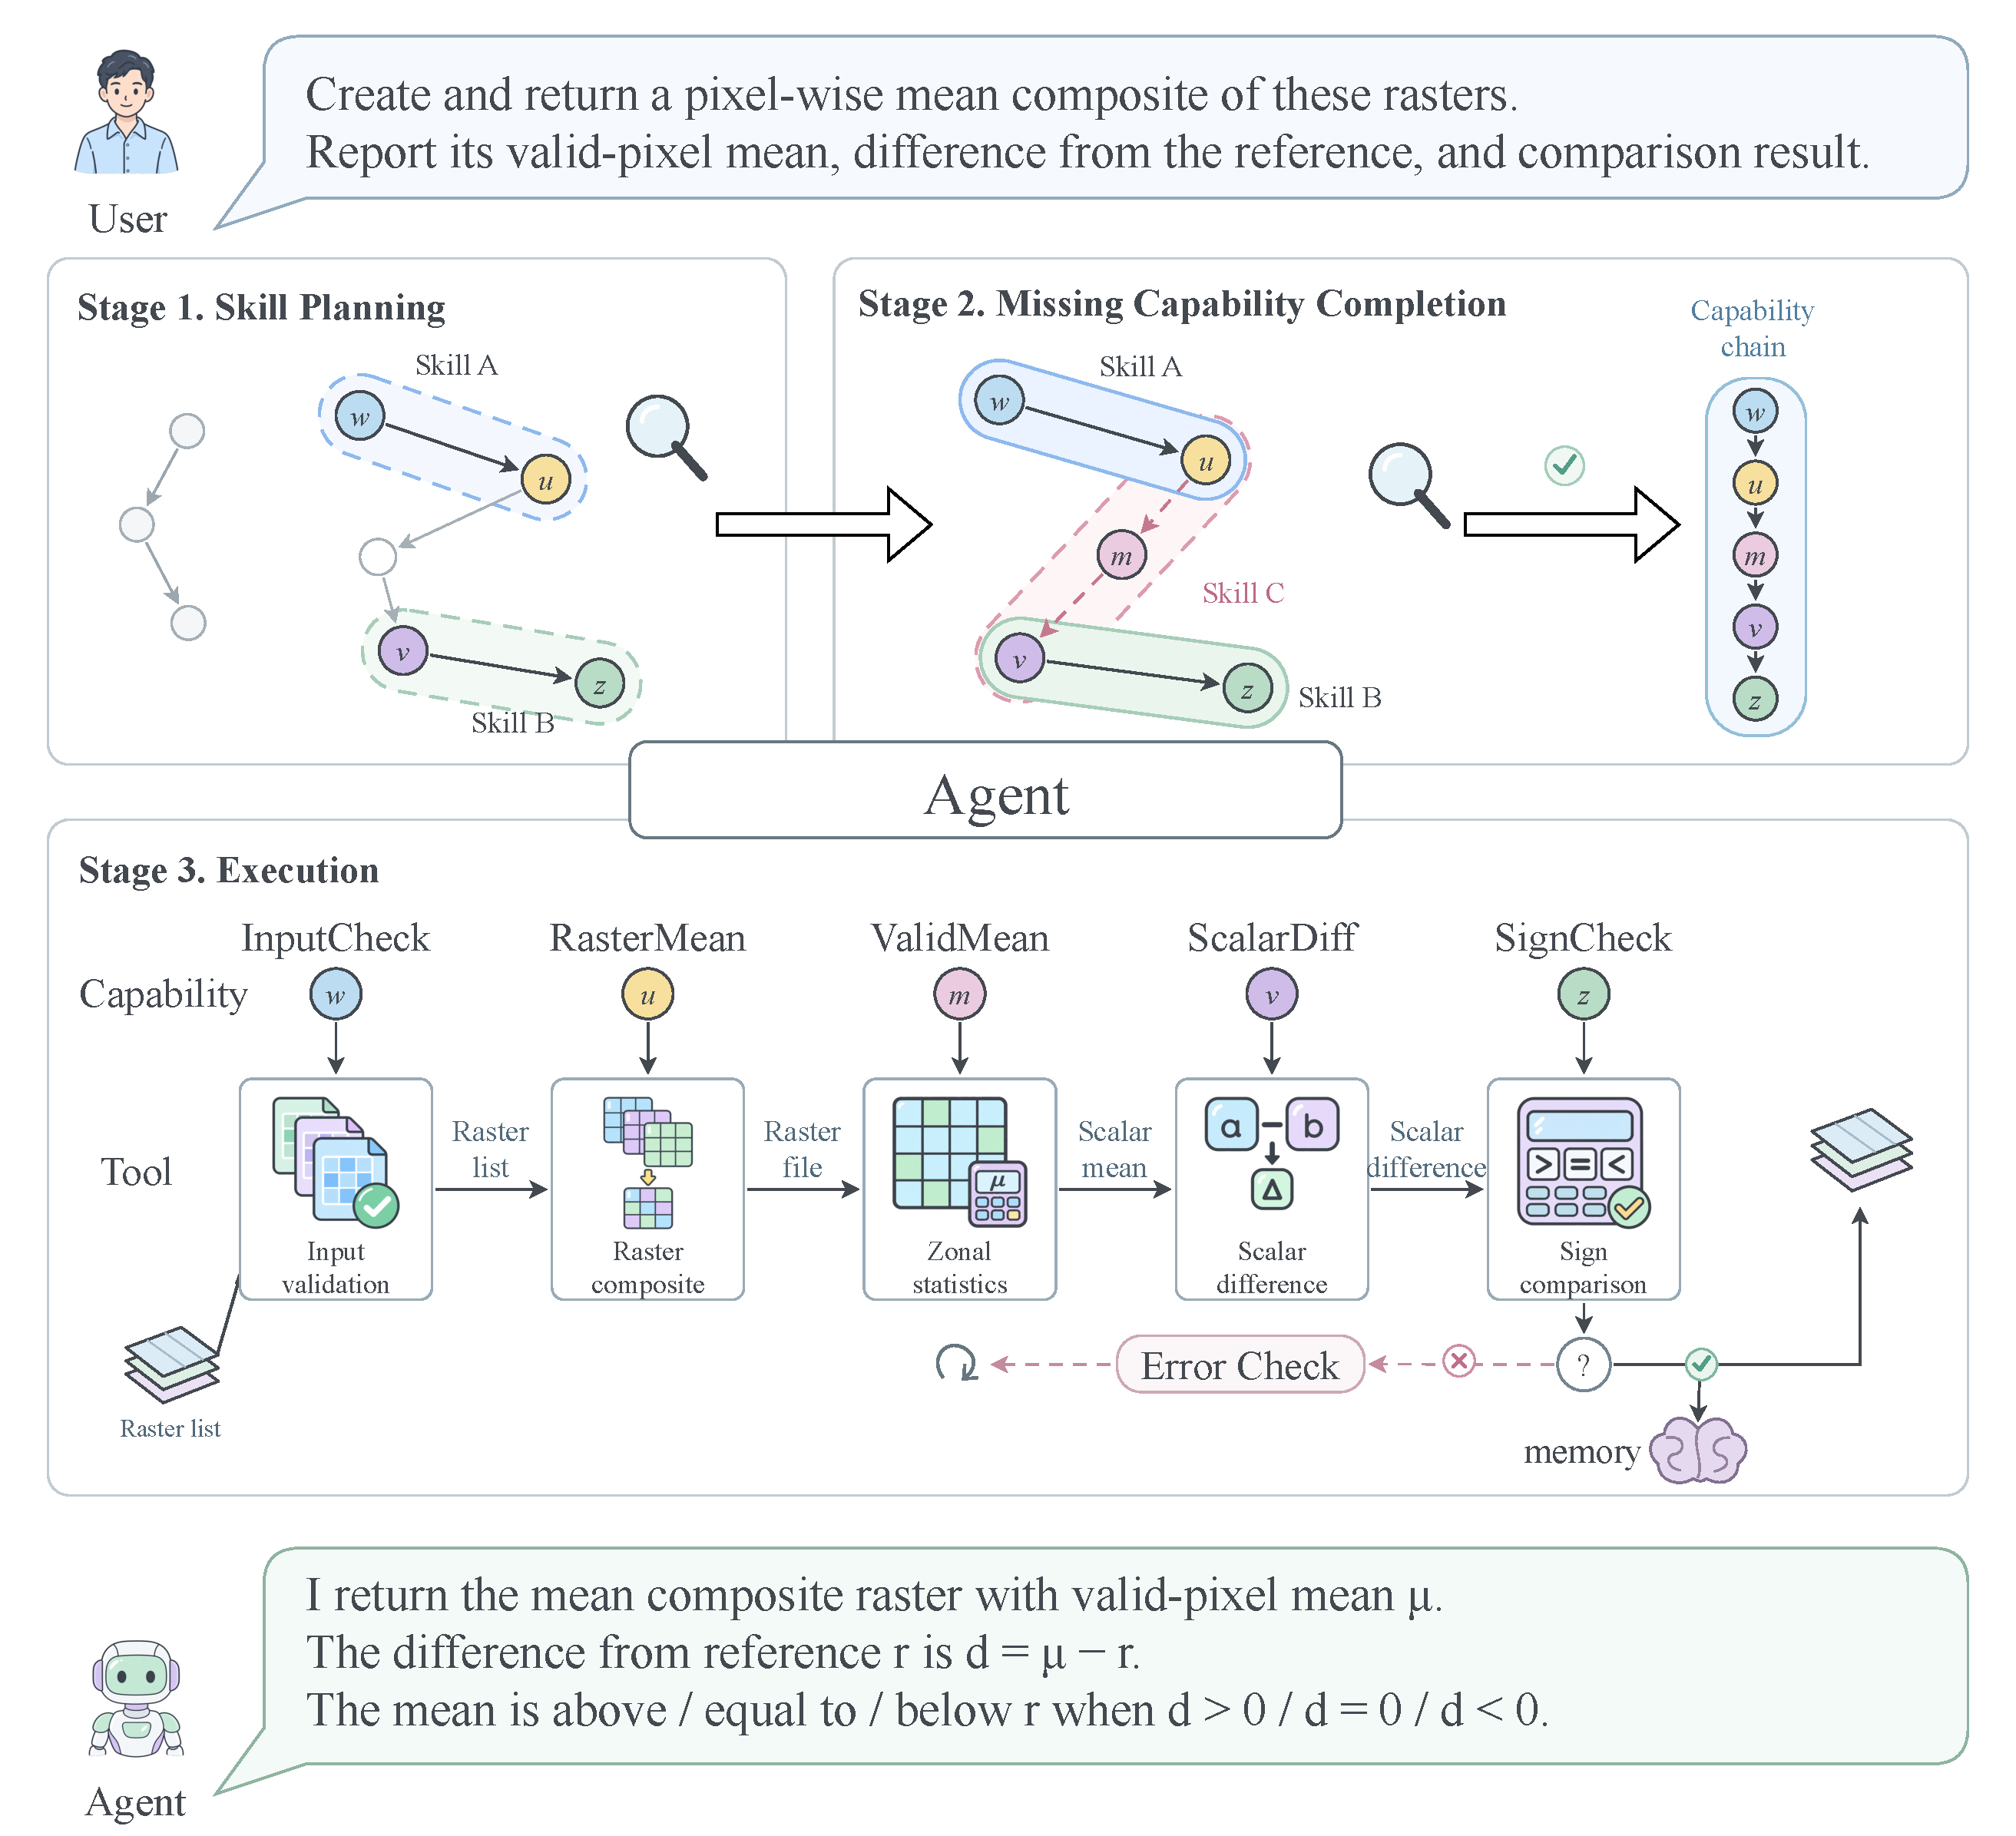
\includegraphics[width=0.83\textwidth]{fig_case_study.pdf}
  \caption{Cross-Skill capability composition and tool execution. Stage 1 selects $w\to u$ from Skill $A$ and $v\to z$ from Skill $B$. Stage 2 inserts valid-pixel mean statistics $m$ using Skill $C$'s $u\to m\to v$ branch. Stage 3 grounds the five-step workflow in tool calls, propagates intermediate artifacts, and returns the composite raster, mean, difference, and comparison relation. The workflow is a mechanism illustration.}
  \label{fig:case-study}
  \Description{The case proceeds from two selected Skill fragments to a completed five-capability chain and corresponding input-validation, raster-compositing, zonal-statistics, scalar-differencing, and sign-comparison tools.}
\end{figure*}


\emph{Skill Retrieval} returns only RasterCompose (Skill $A$) and ReferenceCompare (Skill $B$). \emph{Skill Planning} selects InputCheck ($w$) and RasterMean ($u$) from the former, and ScalarDiff ($v$) and SignCheck ($z$) from the latter. InputCheck verifies the variable and spatial-grid requirements. RasterMean produces the mean raster from the validated image list, giving $w\to u$. ScalarDiff returns the difference between the value under comparison and the reference; SignCheck uses that difference to determine whether the value is above, equal to, or below the reference, giving $v\to z$. Hypergraph Composition expands mandatory predecessors declared by the selected strategies and retains provenance and candidate-tool scopes. At this stage, the plan consists of two disconnected fragments: compositing produces a raster file, whereas differencing requires a numerical input. The operation computing the mean of the composite is still missing.

Using $u$ and $v$ as shared endpoints, Missing Capability Completion retrieves $u\to m\to v$ from inactive RasterDiff (Skill $C$), where ValidMean ($m$) extracts the mean of valid pixels from the composite. Here, RasterDiff means differencing a statistic of the composite against a reference value. The query explicitly requires the mean statistic; Skill $C$ supplies reusable dependencies and usage constraints connecting it to the preceding and following operations. Under this example's assumptions, it is the only candidate for the ordered endpoint pair satisfying prerequisite, type, tool-availability, and acyclicity requirements: $u$'s raster output is compatible with $m$'s input, and $m$'s numerical output is compatible with $v$. Insertion preserves $u$'s original constraints, adds $m$, and updates $v$'s dependencies, candidate-tool scope, and input bindings. Existing dependencies $w\to u$ and $v\to z$ remain. Recomposition and dependency verification connect the fragments into input validation, mean compositing, valid-pixel mean statistics, scalar differencing, and sign comparison: $w\to u\to m\to v\to z$.

Tool Grounding then selects validation, compositing, statistics, differencing, and sign-comparison tools within each instance's candidate scope and parameter constraints. GeoToolKG associations guide candidate retrieval, but concrete invocations still require instance and input-compatibility checks. Grounding a bridge into calls additionally requires that $u$ and $v$ each correspond to exactly one endpoint instance and that their order agrees with the bridge direction. During execution, the validated image list is passed to the compositing tool. The statistics tool receives a list containing only the composite raster's path. The returned mean and the task's reference value are bound to differencing parameters $a$ and $b$, producing $d=a-b$. Sign comparison then compares $d$ with zero. The statistical object remains the composite created for this task, the comparison baseline remains the supplied reference, and the final relation is based on the same difference calculation.

If the zonal-statistics call fails, Failure Recovery uses the failure state and recovery rules to decide whether to retry or select an alternative within the instance's permitted scope. Completed validation and compositing steps are retained, and the composite is reused. Calls with uncertain outcomes are not automatically replayed, and later execution is suspended if recovery requires adding a capability. Once all steps succeed, Final Answer summarizes the composite raster, valid-pixel mean, difference, and comparison relation, addressing each requested output. This case illustrates that cross-Skill completion must both connect capability steps and preserve dependencies while accurately binding task inputs and intermediate artifacts to subsequent calls.

After successful execution and result verification, the five-step workflow can also be organized into a candidate CompositeCompare Skill ($D$). It parameterizes the image list and reference value as rebindable task inputs, and retains artifact dependencies and capability usage constraints. This provides a strategy description for later reuse of the composition. Applicability to other inputs and tasks requires further verification; the example does not establish a reuse benefit for the new Skill.

